\documentclass{standalone}
\usepackage{tikz} % Import the tikz package
\usetikzlibrary{automata} % Import library for drawing automata
\usetikzlibrary{positioning} % ...positioning nodes
\usetikzlibrary{arrows} % ...customizing arrows
\tikzset{node distance=2.5cm,
    every state/.style={
        semithick,
        fill=gray!10},
    initial text={},
    double distance=2pt,
    every edge/.style={
        draw,
        ->,>=stealth',
        auto,
        semithick}}
\let\epsilon\varepsilon
\begin{document}
    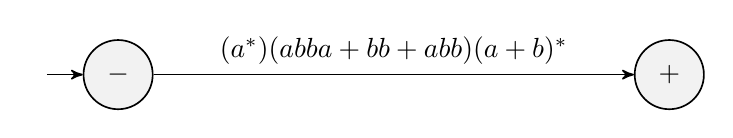
\begin{tikzpicture}
        \node[state,initial] (start) {$-$};
        %\node[state,right of=start] (ul) {$1$};

        %\node[state] (br) at (7,0) {$5$};
        \node[state] (end) at (7,0) {$+$};
        
        \draw (start) edge[] node {$(a^*)(abba+bb+abb)(a+b)^*$} (end);
        %\draw (br) edge[] node {$\Lambda$} (end);
        
        %\draw (ul) edge[loop above] node {\tt a} (ul);

        %\draw (ul) edge[] node {\tt bb + abb + abba} (br);

        %\draw (br) edge[loop below] node {\tt a,b} (br);
    \end{tikzpicture}
\end{document}